
% Default to the notebook output style

    


% Inherit from the specified cell style.




    
\documentclass[11pt]{article}

    
    
    \usepackage[T1]{fontenc}
    % Nicer default font (+ math font) than Computer Modern for most use cases
    \usepackage{mathpazo}

    % Basic figure setup, for now with no caption control since it's done
    % automatically by Pandoc (which extracts ![](path) syntax from Markdown).
    \usepackage{graphicx}
    % We will generate all images so they have a width \maxwidth. This means
    % that they will get their normal width if they fit onto the page, but
    % are scaled down if they would overflow the margins.
    \makeatletter
    \def\maxwidth{\ifdim\Gin@nat@width>\linewidth\linewidth
    \else\Gin@nat@width\fi}
    \makeatother
    \let\Oldincludegraphics\includegraphics
    % Set max figure width to be 80% of text width, for now hardcoded.
    \renewcommand{\includegraphics}[1]{\Oldincludegraphics[width=.8\maxwidth]{#1}}
    % Ensure that by default, figures have no caption (until we provide a
    % proper Figure object with a Caption API and a way to capture that
    % in the conversion process - todo).
    \usepackage{caption}
    \DeclareCaptionLabelFormat{nolabel}{}
    \captionsetup{labelformat=nolabel}

    \usepackage{adjustbox} % Used to constrain images to a maximum size 
    \usepackage{xcolor} % Allow colors to be defined
    \usepackage{enumerate} % Needed for markdown enumerations to work
    \usepackage{geometry} % Used to adjust the document margins
    \usepackage{amsmath} % Equations
    \usepackage{amssymb} % Equations
    \usepackage{textcomp} % defines textquotesingle
    % Hack from http://tex.stackexchange.com/a/47451/13684:
    \AtBeginDocument{%
        \def\PYZsq{\textquotesingle}% Upright quotes in Pygmentized code
    }
    \usepackage{upquote} % Upright quotes for verbatim code
    \usepackage{eurosym} % defines \euro
    \usepackage[mathletters]{ucs} % Extended unicode (utf-8) support
    \usepackage[utf8x]{inputenc} % Allow utf-8 characters in the tex document
    \usepackage{fancyvrb} % verbatim replacement that allows latex
    \usepackage{grffile} % extends the file name processing of package graphics 
                         % to support a larger range 
    % The hyperref package gives us a pdf with properly built
    % internal navigation ('pdf bookmarks' for the table of contents,
    % internal cross-reference links, web links for URLs, etc.)
    \usepackage{hyperref}
    \usepackage{longtable} % longtable support required by pandoc >1.10
    \usepackage{booktabs}  % table support for pandoc > 1.12.2
    \usepackage[inline]{enumitem} % IRkernel/repr support (it uses the enumerate* environment)
    \usepackage[normalem]{ulem} % ulem is needed to support strikethroughs (\sout)
                                % normalem makes italics be italics, not underlines
    

    
    
    % Colors for the hyperref package
    \definecolor{urlcolor}{rgb}{0,.145,.698}
    \definecolor{linkcolor}{rgb}{.71,0.21,0.01}
    \definecolor{citecolor}{rgb}{.12,.54,.11}

    % ANSI colors
    \definecolor{ansi-black}{HTML}{3E424D}
    \definecolor{ansi-black-intense}{HTML}{282C36}
    \definecolor{ansi-red}{HTML}{E75C58}
    \definecolor{ansi-red-intense}{HTML}{B22B31}
    \definecolor{ansi-green}{HTML}{00A250}
    \definecolor{ansi-green-intense}{HTML}{007427}
    \definecolor{ansi-yellow}{HTML}{DDB62B}
    \definecolor{ansi-yellow-intense}{HTML}{B27D12}
    \definecolor{ansi-blue}{HTML}{208FFB}
    \definecolor{ansi-blue-intense}{HTML}{0065CA}
    \definecolor{ansi-magenta}{HTML}{D160C4}
    \definecolor{ansi-magenta-intense}{HTML}{A03196}
    \definecolor{ansi-cyan}{HTML}{60C6C8}
    \definecolor{ansi-cyan-intense}{HTML}{258F8F}
    \definecolor{ansi-white}{HTML}{C5C1B4}
    \definecolor{ansi-white-intense}{HTML}{A1A6B2}

    % commands and environments needed by pandoc snippets
    % extracted from the output of `pandoc -s`
    \providecommand{\tightlist}{%
      \setlength{\itemsep}{0pt}\setlength{\parskip}{0pt}}
    \DefineVerbatimEnvironment{Highlighting}{Verbatim}{commandchars=\\\{\}}
    % Add ',fontsize=\small' for more characters per line
    \newenvironment{Shaded}{}{}
    \newcommand{\KeywordTok}[1]{\textcolor[rgb]{0.00,0.44,0.13}{\textbf{{#1}}}}
    \newcommand{\DataTypeTok}[1]{\textcolor[rgb]{0.56,0.13,0.00}{{#1}}}
    \newcommand{\DecValTok}[1]{\textcolor[rgb]{0.25,0.63,0.44}{{#1}}}
    \newcommand{\BaseNTok}[1]{\textcolor[rgb]{0.25,0.63,0.44}{{#1}}}
    \newcommand{\FloatTok}[1]{\textcolor[rgb]{0.25,0.63,0.44}{{#1}}}
    \newcommand{\CharTok}[1]{\textcolor[rgb]{0.25,0.44,0.63}{{#1}}}
    \newcommand{\StringTok}[1]{\textcolor[rgb]{0.25,0.44,0.63}{{#1}}}
    \newcommand{\CommentTok}[1]{\textcolor[rgb]{0.38,0.63,0.69}{\textit{{#1}}}}
    \newcommand{\OtherTok}[1]{\textcolor[rgb]{0.00,0.44,0.13}{{#1}}}
    \newcommand{\AlertTok}[1]{\textcolor[rgb]{1.00,0.00,0.00}{\textbf{{#1}}}}
    \newcommand{\FunctionTok}[1]{\textcolor[rgb]{0.02,0.16,0.49}{{#1}}}
    \newcommand{\RegionMarkerTok}[1]{{#1}}
    \newcommand{\ErrorTok}[1]{\textcolor[rgb]{1.00,0.00,0.00}{\textbf{{#1}}}}
    \newcommand{\NormalTok}[1]{{#1}}
    
    % Additional commands for more recent versions of Pandoc
    \newcommand{\ConstantTok}[1]{\textcolor[rgb]{0.53,0.00,0.00}{{#1}}}
    \newcommand{\SpecialCharTok}[1]{\textcolor[rgb]{0.25,0.44,0.63}{{#1}}}
    \newcommand{\VerbatimStringTok}[1]{\textcolor[rgb]{0.25,0.44,0.63}{{#1}}}
    \newcommand{\SpecialStringTok}[1]{\textcolor[rgb]{0.73,0.40,0.53}{{#1}}}
    \newcommand{\ImportTok}[1]{{#1}}
    \newcommand{\DocumentationTok}[1]{\textcolor[rgb]{0.73,0.13,0.13}{\textit{{#1}}}}
    \newcommand{\AnnotationTok}[1]{\textcolor[rgb]{0.38,0.63,0.69}{\textbf{\textit{{#1}}}}}
    \newcommand{\CommentVarTok}[1]{\textcolor[rgb]{0.38,0.63,0.69}{\textbf{\textit{{#1}}}}}
    \newcommand{\VariableTok}[1]{\textcolor[rgb]{0.10,0.09,0.49}{{#1}}}
    \newcommand{\ControlFlowTok}[1]{\textcolor[rgb]{0.00,0.44,0.13}{\textbf{{#1}}}}
    \newcommand{\OperatorTok}[1]{\textcolor[rgb]{0.40,0.40,0.40}{{#1}}}
    \newcommand{\BuiltInTok}[1]{{#1}}
    \newcommand{\ExtensionTok}[1]{{#1}}
    \newcommand{\PreprocessorTok}[1]{\textcolor[rgb]{0.74,0.48,0.00}{{#1}}}
    \newcommand{\AttributeTok}[1]{\textcolor[rgb]{0.49,0.56,0.16}{{#1}}}
    \newcommand{\InformationTok}[1]{\textcolor[rgb]{0.38,0.63,0.69}{\textbf{\textit{{#1}}}}}
    \newcommand{\WarningTok}[1]{\textcolor[rgb]{0.38,0.63,0.69}{\textbf{\textit{{#1}}}}}
    
    
    % Define a nice break command that doesn't care if a line doesn't already
    % exist.
    \def\br{\hspace*{\fill} \\* }
    % Math Jax compatability definitions
    \def\gt{>}
    \def\lt{<}
    % Document parameters
    \title{Rascunho modelo}
    
    
    

    % Pygments definitions
    
\makeatletter
\def\PY@reset{\let\PY@it=\relax \let\PY@bf=\relax%
    \let\PY@ul=\relax \let\PY@tc=\relax%
    \let\PY@bc=\relax \let\PY@ff=\relax}
\def\PY@tok#1{\csname PY@tok@#1\endcsname}
\def\PY@toks#1+{\ifx\relax#1\empty\else%
    \PY@tok{#1}\expandafter\PY@toks\fi}
\def\PY@do#1{\PY@bc{\PY@tc{\PY@ul{%
    \PY@it{\PY@bf{\PY@ff{#1}}}}}}}
\def\PY#1#2{\PY@reset\PY@toks#1+\relax+\PY@do{#2}}

\expandafter\def\csname PY@tok@w\endcsname{\def\PY@tc##1{\textcolor[rgb]{0.73,0.73,0.73}{##1}}}
\expandafter\def\csname PY@tok@c\endcsname{\let\PY@it=\textit\def\PY@tc##1{\textcolor[rgb]{0.25,0.50,0.50}{##1}}}
\expandafter\def\csname PY@tok@cp\endcsname{\def\PY@tc##1{\textcolor[rgb]{0.74,0.48,0.00}{##1}}}
\expandafter\def\csname PY@tok@k\endcsname{\let\PY@bf=\textbf\def\PY@tc##1{\textcolor[rgb]{0.00,0.50,0.00}{##1}}}
\expandafter\def\csname PY@tok@kp\endcsname{\def\PY@tc##1{\textcolor[rgb]{0.00,0.50,0.00}{##1}}}
\expandafter\def\csname PY@tok@kt\endcsname{\def\PY@tc##1{\textcolor[rgb]{0.69,0.00,0.25}{##1}}}
\expandafter\def\csname PY@tok@o\endcsname{\def\PY@tc##1{\textcolor[rgb]{0.40,0.40,0.40}{##1}}}
\expandafter\def\csname PY@tok@ow\endcsname{\let\PY@bf=\textbf\def\PY@tc##1{\textcolor[rgb]{0.67,0.13,1.00}{##1}}}
\expandafter\def\csname PY@tok@nb\endcsname{\def\PY@tc##1{\textcolor[rgb]{0.00,0.50,0.00}{##1}}}
\expandafter\def\csname PY@tok@nf\endcsname{\def\PY@tc##1{\textcolor[rgb]{0.00,0.00,1.00}{##1}}}
\expandafter\def\csname PY@tok@nc\endcsname{\let\PY@bf=\textbf\def\PY@tc##1{\textcolor[rgb]{0.00,0.00,1.00}{##1}}}
\expandafter\def\csname PY@tok@nn\endcsname{\let\PY@bf=\textbf\def\PY@tc##1{\textcolor[rgb]{0.00,0.00,1.00}{##1}}}
\expandafter\def\csname PY@tok@ne\endcsname{\let\PY@bf=\textbf\def\PY@tc##1{\textcolor[rgb]{0.82,0.25,0.23}{##1}}}
\expandafter\def\csname PY@tok@nv\endcsname{\def\PY@tc##1{\textcolor[rgb]{0.10,0.09,0.49}{##1}}}
\expandafter\def\csname PY@tok@no\endcsname{\def\PY@tc##1{\textcolor[rgb]{0.53,0.00,0.00}{##1}}}
\expandafter\def\csname PY@tok@nl\endcsname{\def\PY@tc##1{\textcolor[rgb]{0.63,0.63,0.00}{##1}}}
\expandafter\def\csname PY@tok@ni\endcsname{\let\PY@bf=\textbf\def\PY@tc##1{\textcolor[rgb]{0.60,0.60,0.60}{##1}}}
\expandafter\def\csname PY@tok@na\endcsname{\def\PY@tc##1{\textcolor[rgb]{0.49,0.56,0.16}{##1}}}
\expandafter\def\csname PY@tok@nt\endcsname{\let\PY@bf=\textbf\def\PY@tc##1{\textcolor[rgb]{0.00,0.50,0.00}{##1}}}
\expandafter\def\csname PY@tok@nd\endcsname{\def\PY@tc##1{\textcolor[rgb]{0.67,0.13,1.00}{##1}}}
\expandafter\def\csname PY@tok@s\endcsname{\def\PY@tc##1{\textcolor[rgb]{0.73,0.13,0.13}{##1}}}
\expandafter\def\csname PY@tok@sd\endcsname{\let\PY@it=\textit\def\PY@tc##1{\textcolor[rgb]{0.73,0.13,0.13}{##1}}}
\expandafter\def\csname PY@tok@si\endcsname{\let\PY@bf=\textbf\def\PY@tc##1{\textcolor[rgb]{0.73,0.40,0.53}{##1}}}
\expandafter\def\csname PY@tok@se\endcsname{\let\PY@bf=\textbf\def\PY@tc##1{\textcolor[rgb]{0.73,0.40,0.13}{##1}}}
\expandafter\def\csname PY@tok@sr\endcsname{\def\PY@tc##1{\textcolor[rgb]{0.73,0.40,0.53}{##1}}}
\expandafter\def\csname PY@tok@ss\endcsname{\def\PY@tc##1{\textcolor[rgb]{0.10,0.09,0.49}{##1}}}
\expandafter\def\csname PY@tok@sx\endcsname{\def\PY@tc##1{\textcolor[rgb]{0.00,0.50,0.00}{##1}}}
\expandafter\def\csname PY@tok@m\endcsname{\def\PY@tc##1{\textcolor[rgb]{0.40,0.40,0.40}{##1}}}
\expandafter\def\csname PY@tok@gh\endcsname{\let\PY@bf=\textbf\def\PY@tc##1{\textcolor[rgb]{0.00,0.00,0.50}{##1}}}
\expandafter\def\csname PY@tok@gu\endcsname{\let\PY@bf=\textbf\def\PY@tc##1{\textcolor[rgb]{0.50,0.00,0.50}{##1}}}
\expandafter\def\csname PY@tok@gd\endcsname{\def\PY@tc##1{\textcolor[rgb]{0.63,0.00,0.00}{##1}}}
\expandafter\def\csname PY@tok@gi\endcsname{\def\PY@tc##1{\textcolor[rgb]{0.00,0.63,0.00}{##1}}}
\expandafter\def\csname PY@tok@gr\endcsname{\def\PY@tc##1{\textcolor[rgb]{1.00,0.00,0.00}{##1}}}
\expandafter\def\csname PY@tok@ge\endcsname{\let\PY@it=\textit}
\expandafter\def\csname PY@tok@gs\endcsname{\let\PY@bf=\textbf}
\expandafter\def\csname PY@tok@gp\endcsname{\let\PY@bf=\textbf\def\PY@tc##1{\textcolor[rgb]{0.00,0.00,0.50}{##1}}}
\expandafter\def\csname PY@tok@go\endcsname{\def\PY@tc##1{\textcolor[rgb]{0.53,0.53,0.53}{##1}}}
\expandafter\def\csname PY@tok@gt\endcsname{\def\PY@tc##1{\textcolor[rgb]{0.00,0.27,0.87}{##1}}}
\expandafter\def\csname PY@tok@err\endcsname{\def\PY@bc##1{\setlength{\fboxsep}{0pt}\fcolorbox[rgb]{1.00,0.00,0.00}{1,1,1}{\strut ##1}}}
\expandafter\def\csname PY@tok@kc\endcsname{\let\PY@bf=\textbf\def\PY@tc##1{\textcolor[rgb]{0.00,0.50,0.00}{##1}}}
\expandafter\def\csname PY@tok@kd\endcsname{\let\PY@bf=\textbf\def\PY@tc##1{\textcolor[rgb]{0.00,0.50,0.00}{##1}}}
\expandafter\def\csname PY@tok@kn\endcsname{\let\PY@bf=\textbf\def\PY@tc##1{\textcolor[rgb]{0.00,0.50,0.00}{##1}}}
\expandafter\def\csname PY@tok@kr\endcsname{\let\PY@bf=\textbf\def\PY@tc##1{\textcolor[rgb]{0.00,0.50,0.00}{##1}}}
\expandafter\def\csname PY@tok@bp\endcsname{\def\PY@tc##1{\textcolor[rgb]{0.00,0.50,0.00}{##1}}}
\expandafter\def\csname PY@tok@fm\endcsname{\def\PY@tc##1{\textcolor[rgb]{0.00,0.00,1.00}{##1}}}
\expandafter\def\csname PY@tok@vc\endcsname{\def\PY@tc##1{\textcolor[rgb]{0.10,0.09,0.49}{##1}}}
\expandafter\def\csname PY@tok@vg\endcsname{\def\PY@tc##1{\textcolor[rgb]{0.10,0.09,0.49}{##1}}}
\expandafter\def\csname PY@tok@vi\endcsname{\def\PY@tc##1{\textcolor[rgb]{0.10,0.09,0.49}{##1}}}
\expandafter\def\csname PY@tok@vm\endcsname{\def\PY@tc##1{\textcolor[rgb]{0.10,0.09,0.49}{##1}}}
\expandafter\def\csname PY@tok@sa\endcsname{\def\PY@tc##1{\textcolor[rgb]{0.73,0.13,0.13}{##1}}}
\expandafter\def\csname PY@tok@sb\endcsname{\def\PY@tc##1{\textcolor[rgb]{0.73,0.13,0.13}{##1}}}
\expandafter\def\csname PY@tok@sc\endcsname{\def\PY@tc##1{\textcolor[rgb]{0.73,0.13,0.13}{##1}}}
\expandafter\def\csname PY@tok@dl\endcsname{\def\PY@tc##1{\textcolor[rgb]{0.73,0.13,0.13}{##1}}}
\expandafter\def\csname PY@tok@s2\endcsname{\def\PY@tc##1{\textcolor[rgb]{0.73,0.13,0.13}{##1}}}
\expandafter\def\csname PY@tok@sh\endcsname{\def\PY@tc##1{\textcolor[rgb]{0.73,0.13,0.13}{##1}}}
\expandafter\def\csname PY@tok@s1\endcsname{\def\PY@tc##1{\textcolor[rgb]{0.73,0.13,0.13}{##1}}}
\expandafter\def\csname PY@tok@mb\endcsname{\def\PY@tc##1{\textcolor[rgb]{0.40,0.40,0.40}{##1}}}
\expandafter\def\csname PY@tok@mf\endcsname{\def\PY@tc##1{\textcolor[rgb]{0.40,0.40,0.40}{##1}}}
\expandafter\def\csname PY@tok@mh\endcsname{\def\PY@tc##1{\textcolor[rgb]{0.40,0.40,0.40}{##1}}}
\expandafter\def\csname PY@tok@mi\endcsname{\def\PY@tc##1{\textcolor[rgb]{0.40,0.40,0.40}{##1}}}
\expandafter\def\csname PY@tok@il\endcsname{\def\PY@tc##1{\textcolor[rgb]{0.40,0.40,0.40}{##1}}}
\expandafter\def\csname PY@tok@mo\endcsname{\def\PY@tc##1{\textcolor[rgb]{0.40,0.40,0.40}{##1}}}
\expandafter\def\csname PY@tok@ch\endcsname{\let\PY@it=\textit\def\PY@tc##1{\textcolor[rgb]{0.25,0.50,0.50}{##1}}}
\expandafter\def\csname PY@tok@cm\endcsname{\let\PY@it=\textit\def\PY@tc##1{\textcolor[rgb]{0.25,0.50,0.50}{##1}}}
\expandafter\def\csname PY@tok@cpf\endcsname{\let\PY@it=\textit\def\PY@tc##1{\textcolor[rgb]{0.25,0.50,0.50}{##1}}}
\expandafter\def\csname PY@tok@c1\endcsname{\let\PY@it=\textit\def\PY@tc##1{\textcolor[rgb]{0.25,0.50,0.50}{##1}}}
\expandafter\def\csname PY@tok@cs\endcsname{\let\PY@it=\textit\def\PY@tc##1{\textcolor[rgb]{0.25,0.50,0.50}{##1}}}

\def\PYZbs{\char`\\}
\def\PYZus{\char`\_}
\def\PYZob{\char`\{}
\def\PYZcb{\char`\}}
\def\PYZca{\char`\^}
\def\PYZam{\char`\&}
\def\PYZlt{\char`\<}
\def\PYZgt{\char`\>}
\def\PYZsh{\char`\#}
\def\PYZpc{\char`\%}
\def\PYZdl{\char`\$}
\def\PYZhy{\char`\-}
\def\PYZsq{\char`\'}
\def\PYZdq{\char`\"}
\def\PYZti{\char`\~}
% for compatibility with earlier versions
\def\PYZat{@}
\def\PYZlb{[}
\def\PYZrb{]}
\makeatother


    % Exact colors from NB
    \definecolor{incolor}{rgb}{0.0, 0.0, 0.5}
    \definecolor{outcolor}{rgb}{0.545, 0.0, 0.0}



    
    % Prevent overflowing lines due to hard-to-break entities
    \sloppy 
    % Setup hyperref package
    \hypersetup{
      breaklinks=true,  % so long urls are correctly broken across lines
      colorlinks=true,
      urlcolor=urlcolor,
      linkcolor=linkcolor,
      citecolor=citecolor,
      }
    % Slightly bigger margins than the latex defaults
    
    \geometry{verbose,tmargin=1in,bmargin=1in,lmargin=1in,rmargin=1in}
    
    

    \begin{document}
    
    
    \maketitle
    
    

    
    \hypertarget{hipuxf3teses}{%
\section{Hipóteses}\label{hipuxf3teses}}

    \hypertarget{gerais}{%
\subsection{Gerais}\label{gerais}}

\begin{itemize}
\tightlist
\item
  Economia Fehcada e sem governo
\item
  Retornos constantes de escala
\item
  Condições técnicas e produtividade constantes
\item
  Não existem restrições do mercado de trabalho
\item
  Famílias não dividas em classes sociais (simplificação)
\item
  Existe apenas inflação de imóveis
\item
  Não existe depreciação de imóveis
\item
  Exitem quatro setores intitucionais:

  \begin{itemize}
  \tightlist
  \item
    Famílias
  \item
    Firmas
  \item
    Imobiliário
  \item
    Bancos
  \end{itemize}
\item
  Existem apenas três ativos:

  \begin{itemize}
  \tightlist
  \item
    Títulos hipotecários
  \item
    Depósitos à vista
  \item
    Títulos emitidos pelas empresas
  \end{itemize}
\end{itemize}

    \hypertarget{firmas}{%
\subsection{Firmas}\label{firmas}}

\begin{itemize}
\tightlist
\item
  Firmas redistribuem lucros

  \begin{itemize}
  \tightlist
  \item
    Apenas se auferirem lucros
  \end{itemize}
\item
  Firmas financiam investimento com lucros retidos (maior parte),
  empréstimos bancários e emissão de títulos
\item
  Firmas ajustam estoque de capital ao crescimento da demanda efetiva
  (\emph{a lá} supermultiplicador)
\item
  Fixam preços por meio de \emph{mark-up}
\item
  \emph{Mark-up} é definido exogenamente
\item
  Novos empréstimos dependem negativamente da taxa de juros de
  empréstimos
\end{itemize}

    \hypertarget{famuxedlias}{%
\subsection{Famílias}\label{famuxedlias}}

\begin{itemize}
\tightlist
\item
  Consumo depende da renda disponível, depósitos, riqueza financeira
  líquida e rendimentos auferidos pelas residências
\item
  Consumo é fianciado por empréstimos bancários
\item
  Riqueza imobiliária impacta positivamente o colaterál das famílias,
  permitindo contrair mais empréstimos
\item
  Demanda por imóveis pelas famílias depende negativamente da taxa
  própria de juros desses títulos
\end{itemize}

    \hypertarget{setor-imobiliuxe1rio}{%
\subsection{Setor imobiliário}\label{setor-imobiliuxe1rio}}

\begin{itemize}
\tightlist
\item
  Produção de novas resiências se ajusta para atender a demanda
\item
  Imóveis não vendidos afetam negativamente tanto a produção quanto os
  preços
\end{itemize}

    \hypertarget{bancos}{%
\subsection{Bancos}\label{bancos}}

\begin{itemize}
\tightlist
\item
  Taxa dos depósitos à vista são definidos exogenamente
\item
  Bancos concedem empréstimos apenas à agentes suficientemente líquidos
\item
  Parcela dos empréstimos não é paga
\item
  Ajustam liquidez às imposições intitucionais
\item
  Definem taxa de juros de empréstimos como acréscimos da taxa de juros
  de depósitos à vista
\item
  Bancos retém lucros para compensar empréstimos pagos
\end{itemize}

    \hypertarget{matrizes}{%
\section{Matrizes}\label{matrizes}}

    \hypertarget{balanuxe7o-patrimonial}{%
\subsection{Balanço Patrimonial}\label{balanuxe7o-patrimonial}}

    \begin{figure}
\centering
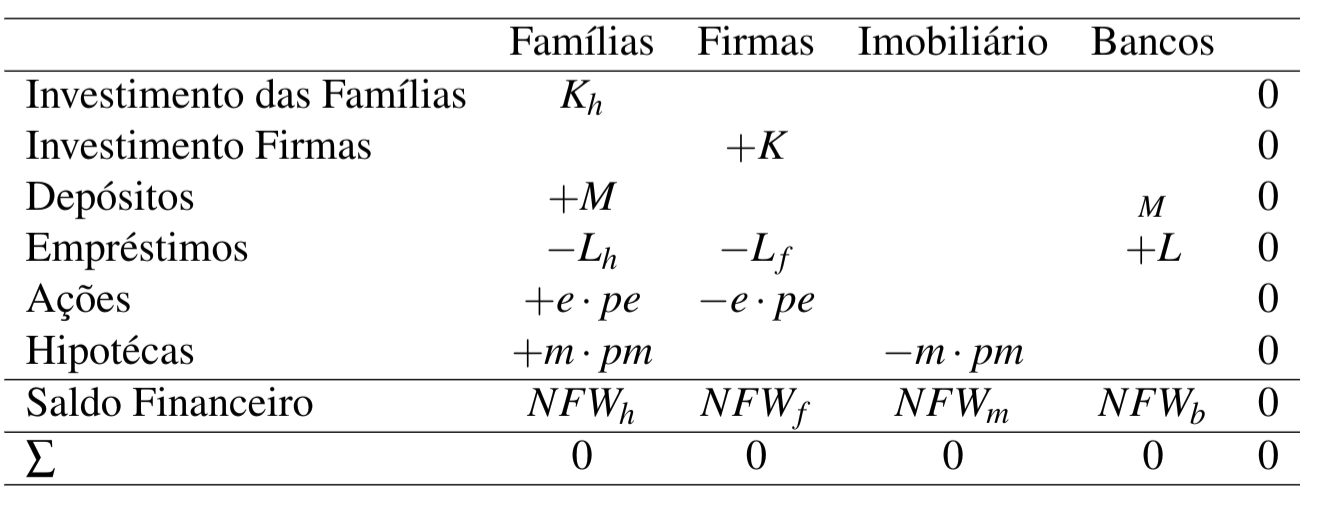
\includegraphics{Patrimonial.png}
\caption{Balanço\_Patrimonial}
\end{figure}

    \hypertarget{matriz-de-reavaliauxe7uxf5es}{%
\subsection{Matriz de reavaliações}\label{matriz-de-reavaliauxe7uxf5es}}

    \begin{figure}
\centering
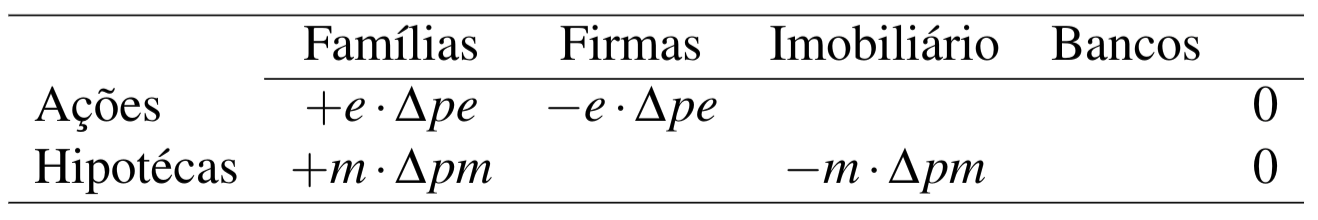
\includegraphics{Reavaliacao.png}
\caption{Reavaliacao}
\end{figure}

    \hypertarget{matriz-de-transauxe7uxf5es}{%
\subsection{Matriz de transações}\label{matriz-de-transauxe7uxf5es}}

    \begin{figure}
\centering
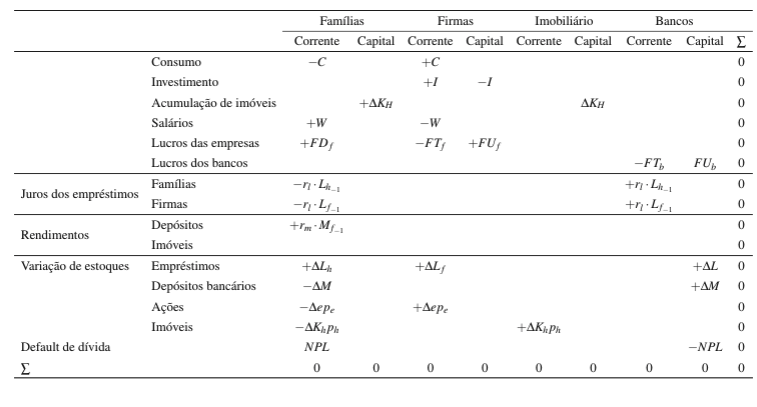
\includegraphics{Transacao.png}
\caption{Matriz de transações}
\end{figure}

    \hypertarget{equauxe7uxf5es-comportamentais}{%
\section{Equações
comportamentais}\label{equauxe7uxf5es-comportamentais}}

    \hypertarget{variuxe1vies}{%
\subsection{Variávies}\label{variuxe1vies}}

\begin{itemize}
\item
  \(Bb_d\) Restrição patrimonial dos bancos
\item
  \(BLR\) Razão de liquidez dos bancos
\item
  \(BUR\) Custo da dívida das famílias em relação à renda disponível
  regular
\item
  \(b\) Produtividade do trabalho
\item
  \(C\) Consumo
\item
  \(CAR\) Taxa de adequação do capital
\item
  \(CG\) Ganhos de Capital
\item
  \(CG_e\) Ganhos de capital com venda de ações
\item
  \(CG_m\) Ganhos de capital com venda de imóveis
\item
  \(Fb\) Lucro total dos bancos
\item
  \(Ff\) Lucro total das Firmas
\item
  \(FD_f\) Lucros distribuídos das firmas
\item
  \(FU_f\) Lucros retido das firmas
\item
  \(F_{fm}\) Lucros do setor imobiliário
\item
  \(GL\) Empréstimo pessoal bruto
\item
  \(g_I\) Taxa de acumulação
\item
  \(g_{If}\) Taxa de crescimento do investimento produtivo
\item
  \(g_{Im}\) Taxa de crescimento do investimento residencial
\item
  \(H^D\) Demanda por imóveis
\item
  \(H^S\) Oferta de imóveis
\item
  \(I\) Investimento agregado
\item
  \(I_f\) Investimento das firmas (Produtivo)
\item
  \(INL\) Imóveis não vendidos (Alterar nome)
\item
  \(I_h\) Investimento residencial
\item
  \(i_m\) Taxa própria de juros dos títulos hipotecários
\item
  \(K\) Estoque de capital fixo
\item
  \(K\) Capital imobiliários
\item
  \(L\) Empréstimos

  \begin{itemize}
  \tightlist
  \item
    \(L_f\) Empréstimos às firmas
  \item
    \(L_h\) Empréstimos às famílias
  \item
    \(L_m\) Empréstimos hipotecários
  \end{itemize}
\item
  \(M\) Depósitos à vista
\item
  \(m\) Títulos hipotecários
\item
  \(N\) Trabalho
\item
  \(NFW_b\) Riqueza financeira líquida dos bancos
\item
  \(NFW_f\) Riqueza financeira líquida das firmas
\item
  \(NFW_h\) Riqueza financeira líquida das famílias
\item
  \(NFW_m\) Riqueza financeira líquida do setor imobiliário
\item
  \(NL\) Empréstimo pessoal líquido
\item
  \(NPL\) Empréstimos não pagos
\item
  \(n\) Crescimento populacional
\item
  \(npl\) Grau de inadimpência
\item
  \(OF\) Fundos dos bancos
\item
  \(p_e\) Preço das ações emitidas pelas firmas
\item
  \(p_m\) Preço dos títulos hipotecários
\item
  \(REP\) Empréstimo quitado (Personal loan repayments) REVER
\item
  \(r_k\) Rendimento dos dividendos das firmas
\item
  \(r_l\) Taxa de juros dos empréstimos
\item
  \(r_m\) Taxa de rendimento dos depósitos à vista
\item
  \(spread\) \emph{spread} sobre a taxa de depósitos
\item
  \(v\) Relação técnica capital-Produto normal
\item
  \(V_{fma}\) Ativos de mercado financeiro
\item
  \(u\) Grau de utilização da capacidade
\item
  \(W\) Salários
\item
  \(Y\) Produto
\item
  \(Y_{fc}\) Produto potencial
\item
  \(Yh\) Renda das Famílias
\item
  \(YD_r\) Renda regular disponível das famílias
\item
  \(YD_{cg}\): Renda disponível com ganhos de capital (Haig-Simons)
\item
  \(Z\) Gastos autônomos não criadores de capacidade
\item
  \(\alpha_1\) Propensão marginal à consumir à partir da renda
\item
  \(\alpha_2\) Propensão marginal à consumir à partir da riqueza
  financeira
\item
  \(\beta_m\) Correção expectacional
\item
  \(\delta_m\) Taxa de amortização do empréstimo hipotecário
\item
  \(\eta\) Razão entre novos empréstimos e renda das famílias
\item
  \(\gamma^e\) Taxa de crescimento esperada de imóveis (alterar nome)
\item
  \(\gamma_m\) Propensão à especular com imóveis
\item
  \(\mu\) Mark-up
\item
  \(\omega\) Participação dos salários na renda
\item
  \(\pi\) Participação dos lucros na renda
\item
  \(\phi\) Valor de entrada no empréstimo imobiliário
\item
  \(\pi_m\) Inflação de imóveis
\item
  \(\Psi\) Parcela dos lucros distribuídos das firmas
\end{itemize}

    \hypertarget{gerais}{%
\subsection{Gerais}\label{gerais}}

\[
Y = \min \{vK, bN\} \Rightarrow Y = vK
\]

\[
Y = C + I
\]

\[
W = \omega Y
\]

\[
\omega = 1-\pi
\]

\[
\pi = \frac{\mu}{1+\mu}
\]

\[
F = Y - W
\]

\[
F = FU_f + Fb 
\]

\[
I = I_f + H
\]

\[
Z = H + NL
\]

\[
Y_{fc} = \frac{K_{-1}}{v}
\]

\[
u = \frac{Y}{Y_{fc}}
\]

    \hypertarget{famuxedlias}{%
\subsection{Famílias}\label{famuxedlias}}

\[
Yh = W + FD_f + r_{m_{-1}}\cdot M 
\]

\[
YD_r = Yh - r_{l{-1}}L_{h_{-1}} - i_mL_{m_{-1}}
\]

\[
YD_{cg} = YD_r + CG
\]

\[
CG = CG_m
\]

\[
CG_m = \Delta p_m - \delta_m L_{m_{-1}}
\]

\[
C = \alpha_1(YD_r + NL) + \alpha_2 NFW_h
\]

\[
H^D = \Xi + \gamma_m (1- i_m)H^D_{-1}
\]

\[
i_m = \frac{1+m}{1+\pi_m} - 1
\]

\[
\Delta NFW_h = YD_{cg} - C
\]

\[
GL = \eta YD_r
\]

\[
\eta = \eta_0 -\eta_rrl
\]

\[
NL = GL
\]

\[
\Delta L_h = NL  - CG
\]

\[
\Delta L_m = \phi p_m + (1-\delta_m) L_{m_{-1}} 
\]

\[
BUR = \frac{r_{l_{-1}}\cdot L_{h_{-1}} + i_m\cdot L_{m_{-1}}}{YDr}
\]

    \hypertarget{alocauxe7uxe3o-de-portfuxf3lio}{%
\subsubsection{Alocação de
portfólio}\label{alocauxe7uxe3o-de-portfuxf3lio}}

\[
V_{fma} = M + p_e\cdot e + p_m\cdot m \Leftrightarrow L_h + NFW_h = V_{fma}
\]

\[
r_k = \frac{FD_f}{e_{-1}\cdot p_{e_{-1}}}
\]

    \hypertarget{firmas}{%
\subsection{Firmas}\label{firmas}}

\[
I_f = hY
\]

\[
K = K_{-1} + I_f - \delta K_{-1}
\]

\[
L_f = L_{f_{-1}} + I_f - FU_f - pe\Delta e
\]

\[
h = h_{-1}\gamma (u - u_n)
\]

\[
F_f = F - Fb - F_{fm}
\]

\[
FU_f = Ff - FD_f - r_l\cdot L_{f_{-1}}
\]

\[
FD_f = \Psi Ff
\]

\[
\Delta L_f = I - FU_f - \Delta e \cdot pe
\]

    \hypertarget{setor-imobiliuxe1rio}{%
\subsection{Setor imobiliário}\label{setor-imobiliuxe1rio}}

\[
H^S = (1+\gamma^e )\overbrace{(H^S_{-1} - INL_{-1})}^{H^D_{-1}}
\]

\[
\gamma^e = \gamma^e_{-1} +\beta (g_{Ih_{-1}} - \gamma^e_{-1})
\]

\[
INL = H^S - H^D
\]

\[
\Delta p_m = ????
\]

    \hypertarget{bancos}{%
\subsection{Bancos}\label{bancos}}

\[
M^S = M^D
\]

\[
i_m = \overline i_m
\]

\[
Bb_d = M^S - L_f^S - L_h^S 
\]

\[
BLR = \frac{Bb_{d}}{M^S}
\]

\[
\Delta r_m = \xi (\xi_1 - \xi_2)
\]

\[
\xi_2 = 
\begin{cases}
1 \text{ se } BLR < \text{piso}\\
0 \,\,\,\,\,\,\, \text{c.c.}
\end{cases}
\]

\[
\xi_1 = 
\begin{cases}
1 \text{ se } BLR > \text{teto}\\
0 \,\,\,\,\,\,\, \text{c.c.}
\end{cases}
\]

\[
rl = rm + \overline{spread}
\]

\[
Fb = rl_{-1}L - rm_{-1}M
\]

    \hypertarget{soluuxe7uxf5es-analuxedticas}{%
\section{Soluções analíticas}\label{soluuxe7uxf5es-analuxedticas}}

    \hypertarget{simulauxe7uxf5es}{%
\section{Simulações}\label{simulauxe7uxf5es}}

    \hypertarget{choques}{%
\section{Choques}\label{choques}}

    \hypertarget{anuxe1lise-dos-resultados}{%
\section{Análise dos resultados}\label{anuxe1lise-dos-resultados}}


    % Add a bibliography block to the postdoc
    
    
    
    \end{document}
